\documentclass[11pt,a4paper]{article}

\usepackage[T1]{fontenc}
\usepackage[utf8]{inputenc}
\usepackage{lmodern}
\usepackage{microtype}
\usepackage[margin=25mm]{geometry}
\usepackage{setspace}
\usepackage{graphicx}
\usepackage{booktabs}
\usepackage{tabularx}
\usepackage{array}
\usepackage{threeparttable}
\usepackage{multirow}
\usepackage{amsmath,amssymb}
\usepackage{siunitx}
\usepackage{enumitem}
\usepackage{xcolor}
\usepackage{tikz}
\usetikzlibrary{arrows.meta,positioning,fit,shapes.geometric}
\usepackage{pgfplots}
\pgfplotsset{compat=1.18}
\usepackage[round,authoryear]{natbib}
\usepackage[hidelinks]{hyperref}
\usepackage{xurl}
\usepackage[nameinlink,noabbrev]{cleveref}
\usepackage{fancyhdr}
\usepackage{caption}
\usepackage{subcaption}
\usepackage{float}
\usepackage{listings}

\newcommand{\reporttitle}{SkinSmith: A Constraint-Aware Generative Agent for Game Weapon Skin Design - A Counter-Strike 2 Case Study}
\newcommand{\registeredtopic}{Latent Vision $\rightarrow$ Image Generation}
\newcommand{\studentname}{YUAN Ye}
\newcommand{\reportauthors}{YUAN Ye, CHEN Yuhong, Ben Tangjie, Wang Zhengye, WANG Lihui}
\newcommand{\supervisor}{Prof. Yu Yang}
\newcommand{\submissiondate}{2 August 2026}
\newcommand{\repositoryurl}{https://github.com/DID-FIELD/SDSC6002-SkinSmith}
\newcommand{\memberone}{YUAN Ye}
\newcommand{\memberoneid}{60089337}
\newcommand{\membertwo}{CHEN Yuhong}
\newcommand{\membertwoid}{59877861}
\newcommand{\memberthree}{Ben Tangjie}
\newcommand{\memberthreeid}{59341974}
\newcommand{\memberfour}{Wang Zhengye}
\newcommand{\memberfourid}{59928724}
\newcommand{\memberfive}{WANG Lihui}
\newcommand{\memberfiveid}{59252928}


\definecolor{skinsmithblue}{HTML}{1565C0}
\definecolor{skinsmithteal}{HTML}{008C95}
\definecolor{skinsmithdark}{HTML}{263238}
\definecolor{skinsmithlight}{HTML}{EEF4F8}

\hypersetup{
  pdftitle={\reporttitle},
  pdfauthor={\reportauthors},
  pdfsubject={SDSC6002 Research Project},
  colorlinks=true,
  linkcolor=skinsmithblue,
  citecolor=skinsmithteal,
  urlcolor=skinsmithblue
}

\pagestyle{fancy}
\fancyhf{}
\lhead{\small SkinSmith}
\rhead{\small SDSC6002 Research Project}
\cfoot{\thepage}
\setlength{\headheight}{14pt}
\onehalfspacing
\setlength{\parskip}{0.35em}
\setlength{\parindent}{1.5em}
\setlist{nosep}
\graphicspath{{figures/}}
\sisetup{round-mode=places,round-precision=4,detect-all}

\newcommand{\routeA}{Route~A}
\newcommand{\routeB}{Route~B}
\newcommand{\routeC}{Route~C}
\newcommand{\skinsmith}{SkinSmith}
\newcommand{\assetseam}{E_{\mathrm{asset}}}
\newcommand{\multiview}{S_{\mathrm{view}}}

\begin{document}

\pagenumbering{gobble}
\begin{titlepage}
  \centering
  \vspace*{18mm}
  {\Large City University of Hong Kong\par}
  \vspace{4mm}
  {\large Master of Science in Data Science\par}
  \vspace{22mm}
  {\Huge\bfseries \reporttitle\par}
  \vspace{9mm}
  {\large Registered Project Topic: \registeredtopic\par}
  \vspace{5mm}
  {\Large SDSC6002 Research Project\par}
  \vfill
  \begin{tabular}{ll}
    \toprule
    \textbf{Group member} & \textbf{Student ID}\\
    \midrule
    \memberone & \memberoneid\\
    \membertwo & \membertwoid\\
    \memberthree & \memberthreeid\\
    \memberfour & \memberfourid\\
    \memberfive & \memberfiveid\\
    \bottomrule
  \end{tabular}
  \vspace{8mm}

  \begin{tabular}{rl}
    Supervisor: & \supervisor\\
    Submission date: & \submissiondate
  \end{tabular}
  \vfill
  {\small This report describes an academic prototype. Counter-Strike 2 is used
  as a case study; the project is not affiliated with Valve and does not publish
  items to the Steam Workshop.\par}
\end{titlepage}

\clearpage
\pagenumbering{roman}
\begin{abstract}
Text-to-image models produce rectangular images, whereas a usable game-asset
texture must remain coherent after it is cut into a fragmented UV atlas, mapped
onto a narrow three-dimensional surface, viewed from several directions, and
exported under asset-specific constraints. This report presents \skinsmith, a
human-supervised generative Agent that converts a short theme keyword into a
mapped and reproducible weapon texture. The system introduces three checkpoints:
the user confirms an expanded visual theme, selects one textual art direction,
and selects one artwork only after seeing its source image together with left,
right, and top weapon previews.

The technical method separates a tileable-pattern baseline from a weapon-aware
route. The latter derives a canonical coordinate frame from the target mesh,
constructs per-UV-pixel position and normal maps, fits a selected master artwork
to continuous weapon-space canvases, and then bakes the result into the asset's
existing UV atlas. Candidates are evaluated using texture statistics, a
mesh-derived seam metric, and fixed multi-view renders. Selection first enforces
hard constraints and then applies Pareto dominance and a deterministic objective
order. One local refinement round is permitted, but it is retained only when it
improves the locked score by at least 0.01; otherwise the system rolls back.

In a four-pair formal experiment on an AK-47 asset, the weapon-space route reduced
asset-seam error by a mean of 0.2693 and improved the multi-view score by 0.0601,
winning all four paired comparisons on both measures. A separate selection-policy
ablation showed that an equal weighted score chose an infeasible seam width,
whereas constraint-first selection returned a valid operating point. All four
formal refinement attempts were rejected and rolled back, demonstrating bounded
no-regression behavior rather than guaranteed self-improvement. A real
three-checkpoint run generated four mapped artwork alternatives from the keyword
\emph{dragon}; the user-selected candidate was exported as a 2048 by 2048 RGB
texture with asset-seam error 0.00078 and multi-view score 0.8166. Transfer to an
M4A4 adapter reused the core pipeline without new image generation, but did not
satisfy the AK-47 retention threshold, exposing the asset-specific limits of
portability.

The results support the value of composing and evaluating artwork in the target
asset's geometry rather than treating image generation as the final output. They
also show why human selection, explicit feasibility rules, preserved evidence,
and rollback are necessary in a creative Agent whose automatic metrics remain
imperfect.
\end{abstract}

\tableofcontents
\clearpage
\listoffigures
\listoftables
\clearpage

\pagenumbering{arabic}
\section{Introduction}
\label{sec:introduction}

\subsection{Problem context}

Generative image models have made it straightforward to produce visually rich
concept art from a short text prompt. That capability does not, by itself, solve
the problem of designing a texture for an existing three-dimensional game asset.
The visible surface of a weapon is stored as a set of UV charts: pieces of the
surface are flattened, rotated, scaled, and packed into a square image. A source
illustration that looks coherent in two dimensions can therefore be split across
unrelated atlas regions, disappear on narrow components, or become inconsistent
between the left, right, and top views. Export requirements, paintable regions,
texture resolution, and seam behavior add further constraints.

This distinction matters for both research and practice. If the generated source
image is treated as the result, an evaluation can reward an attractive rectangle
while overlooking the failures introduced by mapping. Conversely, a simple
tileable pattern may survive arbitrary UV fragmentation but provide little control
over whole-weapon composition. A useful system must connect creative generation to
the actual asset contract and must make its decisions observable.

\skinsmith\ addresses this integration problem. It is a constraint-aware
generative Agent for weapon-skin design, evaluated through a Counter-Strike 2
case study. The system accepts a registered weapon and a compact theme such as
\emph{dragon}. It expands the theme into a visual world, offers several textual
directions, generates several landscape artworks for the selected direction, and
maps every artwork to the target geometry before asking the user to choose. The
chosen source is then processed at full resolution, evaluated, optionally refined
once, and exported with prompts, model identifiers, hashes, metrics, and decisions.

\subsection{Scope}

The research object is the Agent workflow and its geometry-aware texture pipeline,
not a universal Counter-Strike skin generator. The AK-47 is the complete case
study. An M4A4 adapter is used to examine transfer, but it is not presented as an
equivalent production result. The system preserves each asset's existing UV
layout; it does not perform automatic UV unwrapping. Its software renderer provides
controlled technical views rather than photorealistic game-engine rendering.
Steam Workshop publication is outside the project scope.

The group originally registered under the umbrella topic
\emph{Latent Vision $\rightarrow$ Image Generation}. Its initial brief proposed a
broad investigation of image-to-image generation, diffusion models, prompt
engineering, conditioning, and creative outputs such as illustrations, game
concept art, and posters. With fewer than three weeks remaining, the supervisor
advised the group to narrow the work to the technical development of a completed
image-processing Agent and explicitly stated that it did not need to remain the
original broad Latent Vision project. \skinsmith\ is the resulting scoped research
project: it retains image generation and human-AI collaboration from the registered
topic, but concentrates them on one technically testable asset pipeline.

This approved narrowing made it possible to evaluate the complete path from intent
to deployable texture, including negative results, UV failures, selection errors,
and rollback behavior that would be invisible in a source-image-only study. The
registered topic is therefore retained on the title page for administrative
continuity, while the report title names the actual system and research question.

\subsection{Research questions}

The study addresses five questions:

\begin{description}[leftmargin=1.2cm,style=nextline]
  \item[RQ1] Does composing artwork in a mesh-derived continuous weapon space and
  then baking it to the authoritative UV atlas improve mapped asset-seam and
  multi-view performance relative to a generic tileable-pattern baseline?

  \item[RQ2] What failures become observable when candidates are evaluated after
  mapping to the real weapon from left, right, and top views rather than only as
  source images or flat texture atlases?

  \item[RQ3] Can hard-constraint filtering, Pareto-based selection, and a bounded
  correction with rollback prevent an Agent from accepting technically invalid or
  lower-quality updates that a soft aggregate score might prefer?

  \item[RQ4] Can three explicit human checkpoints separate theme intent,
  art-direction choice, and mapped-artwork selection while allowing the Agent to
  begin from one short keyword?

  \item[RQ5] Which parts of the pipeline transfer to a second weapon through a
  \texttt{GameAssetAdapter}, and which geometry, material, camera, and deployment
  contracts remain asset-specific?
\end{description}

\subsection{Contributions}

The project makes five bounded contributions:

\begin{enumerate}
  \item A weapon-space-to-UV generation route that composes selected artwork in a
  canonical frame derived from the target mesh and bakes it through per-UV-pixel
  geometry maps into the existing atlas.
  \item Render-in-the-loop evaluation in which source images, true asset seams,
  and fixed left, right, and top renders are retained as separate evidence.
  \item A small-pool multi-objective policy that separates feasibility from
  preference and permits one local correction with an explicit rollback gate.
  \item A three-checkpoint human-Agent interaction that preserves human authority
  over the theme, direction, and mapped artwork.
  \item An adapter boundary that distinguishes reusable planning and evaluation
  logic from asset-specific mesh, UV, camera, and export contracts.
\end{enumerate}

These claims concern the integration and evaluation of a deployable workflow.
They do not claim the first use of diffusion for mesh texturing, the first
multi-view texture method, or general compatibility with every game asset.

\subsection{Report structure}

\Cref{sec:related} positions the work against diffusion, texture synthesis,
3D-aware texturing, constrained selection, and human-AI systems.
\Cref{sec:method} describes the Agent, asset representation, weapon-space bake,
evaluation, and refinement rules. \Cref{sec:experiments} defines the controlled
experiments and evidence protocol. \Cref{sec:results} reports findings in the
order of the research questions. \Cref{sec:discussion} considers validity,
limitations, project management, and responsible use before
\cref{sec:conclusion} concludes.

\section{Related Work}
\label{sec:related}

\subsection{Image generation and structural control}

Diffusion models learn to reverse a gradual noising process and provide a stable
foundation for high-quality image synthesis \citep{ho2020ddpm}. Improved
parameterizations and sampling methods made the approach more efficient
\citep{nichol2021improved}, while latent diffusion reduced the cost of
high-resolution synthesis by operating in a learned latent space
\citep{rombach2022latent}. Joint image-text representations such as CLIP enabled
general semantic comparison between prompts and images \citep{radford2021clip}.
These developments explain why an existing image model can serve as a strong
source-art generator in \skinsmith.

The limitation is spatial control. A text prompt can describe a dragon, cloud, or
metallic surface, but it does not specify how those elements should survive a
particular UV atlas. ControlNet demonstrates the broader value of supplementing
text with spatial conditions such as edges, depth, and segmentation
\citep{zhang2023controlnet}. \skinsmith\ adopts the same motivation without
training a new conditioning network: semantic planning is separated from
deterministic geometry-based placement and evaluation.

\subsection{Texture synthesis, periodicity, and UV atlases}

Classical texture-synthesis methods grow or assemble images from local
neighborhoods and patches \citep{efros1999texture,efros2001quilting}. Graph-cut
textures improve joins between overlapping patches by optimizing the cut through
the overlap \citep{kwatra2003graphcut}. Periodic-plus-smooth decomposition
addresses discontinuities caused when a finite image is treated as periodic in
the Fourier domain \citep{moisan2011periodic}. This work supports the use of a
tileable pattern as a meaningful baseline and motivates the frequency-domain
border repair used by \routeA.

Square-border periodicity is nevertheless different from continuity on a mesh.
Surface parameterization flattens a three-dimensional surface into one or more
charts and must trade distortion against chart layout
\citep{floater2005parameterization}. Least-squares conformal maps are a widely
used approach to low-angle-distortion atlases, but chart boundaries still
interrupt large regular patterns \citep{levy2002lscm}. TextureMontage further
shows that positioning multiple images on an arbitrary surface requires explicit
control over distortion and transitions \citep{zhou2005texturemontage}. In a game
pipeline, the UV contract is often already fixed. \skinsmith\ therefore does not
replace the parameterization; it derives geometry maps and seam correspondences
from the bound asset and works within that atlas.

\subsection{Diffusion-based 3D texturing}

Several systems use two-dimensional diffusion priors to generate appearance for
three-dimensional objects. DreamFusion demonstrated that rendered views can
connect a text-to-image prior to a 3D representation without a large paired 3D
dataset \citep{poole2022dreamfusion}. TEXTure progressively paints an existing
mesh from depth-conditioned views and supports text-guided generation and editing
\citep{richardson2023texture}. Text2Tex similarly uses a progressive
generate-and-refine process with view partitioning and automatic view selection
\citep{chen2023text2tex}. TexFusion aggregates denoising predictions in a shared
latent texture representation to improve global consistency
\citep{cao2023texfusion}. Point-UV Diffusion combines a low-frequency point-space
representation with UV-space refinement \citep{yu2023pointuv}. Paint3D adds UV
inpainting and high-resolution refinement to produce complete, lighting-less
texture maps \citep{zeng2024paint3d}. Synchronized multi-view diffusion shares
denoised content between overlapping views during sampling
\citep{liu2024syncmvd}.

This literature establishes that UV discontinuity, view inconsistency,
incomplete coverage, and baked illumination are central problems. It also limits
the novelty claim that can reasonably be made here: \skinsmith\ is not the first
system to texture a mesh using diffusion. Its focus is a different layer of the
problem---an asset-bound, human-supervised Agent that begins with compact intent,
retains the target game's UV contract, exposes mapped alternatives before formal
execution, enforces deployment constraints, and preserves the evidence behind
every decision.

\begin{table}[t]
  \centering
  \caption{Positioning against the closest 3D-texturing systems. ``Not central''
  means that the property is not a principal reported contribution, not that an
  extension would be impossible.}
  \label{tab:closest-work}
  \small
  \begin{tabularx}{\textwidth}{p{1.8cm} X X X}
    \toprule
    Work & Main mechanism & Consistency and UV treatment & Human and deployment control\\
    \midrule
    TEXTure & Iterative depth-conditioned painting & Successive views are projected
    to a mesh texture & Text-guided generation and editing; hard deployment gates
    are not central\\
    Text2Tex & Progressive generation and refinement & View partitioning and
    automatic next-view selection update visible texels & Prompt-controlled; no
    explicit rollback contract reported\\
    TexFusion & Shared latent texture denoising & View predictions are aggregated
    on one latent texture & Text-conditioned; no staged human checkpoint contract\\
    Point-UV & Point-space coarse colour followed by UV diffusion & Low-frequency
    global condition plus UV refinement & Conditional generation; no game-specific
    export gate\\
    Paint3D & Multi-view fusion, UV inpainting, and UVHD refinement & Complete
    high-resolution lighting-less UV maps & Text or image conditioning; focuses on
    texture quality rather than Agent rollback\\
    SyncMVD & Synchronized denoising across overlapping views & Shares latent
    content at each denoising step & Text-guided; no three-stage selection contract\\
    \skinsmith & User-selected master artwork and deterministic weapon-space bake &
    Preserves the authoritative UV; evaluates fixed mapped views and true seams &
    Three checkpoints, hard feasibility, one bounded correction, and rollback\\
    \bottomrule
  \end{tabularx}
\end{table}

\subsection{Rendering and evaluation}

Differentiable rendering research formalizes the link between a 3D representation
and image-space supervision \citep{kato2018renderer,liu2019softras}. \skinsmith\
does not optimize through rendering gradients, but follows the same general
principle: the mapped views are evidence about the texture that cannot be recovered
from the source image alone.

Perceptual metrics also require care. LPIPS showed that learned feature distances
often correlate with human perceptual judgments better than simple pixel
distances \citep{zhang2018lpips}. CLIPScore provides reference-free semantic
compatibility, while documenting cases in which such a score is weaker
\citep{hessel2021clipscore}. Accordingly, \skinsmith\ keeps texture, seam,
multi-view, and semantic evidence separate. Automated review recommends and
explains; it does not replace artwork selection by the user.

\subsection{Constrained selection and bounded Agents}

Weighted aggregation is convenient, but a high score on one objective can hide a
violation on another. Feasibility-oriented constraint handling instead ranks
valid solutions ahead of invalid ones \citep{deb2000constraints}. NSGA-II
formalizes non-dominated sorting for multi-objective optimization
\citep{deb2002nsgaii}. \skinsmith\ adapts these principles to a small, expensive
candidate pool rather than running an evolutionary search: it filters hard
violations, computes the feasible Pareto set, and uses a fixed objective order.

Agent research provides a second relevant foundation. ReAct interleaves reasoning
and actions so observations can change the trajectory \citep{yao2023react}.
Self-Refine and Reflexion use feedback and memory to improve later attempts without
updating model weights \citep{madaan2023selfrefine,shinn2023reflexion}. These
methods motivate explicit observation, diagnosis, action, and memory, but they do
not imply that every revision is better. \skinsmith\ therefore limits refinement
to one local round and requires measured improvement before acceptance.

\subsection{Human control and responsible generation}

Human-AI interaction guidelines emphasize communicating capabilities, allowing
correction, and preserving user control when model behavior is uncertain
\citep{amershi2019guidelines}. Co-creative systems treat generation as a turn-based
collaboration \citep{guzdial2019cocreative}, while PromptChainer demonstrates the
value of visible intermediate stages for complex AI tasks
\citep{wu2022promptchainer}. These ideas inform the three checkpoints in
\skinsmith: theme, direction, and mapped artwork.

Finally, datasheets and model cards show why provenance, intended use, evaluation
conditions, and limitations should be recorded
\citep{gebru2021datasheets,mitchell2019modelcards}. Responsible-AI scholarship
also warns that fluent outputs can obscure data, bias, environmental, and
accountability concerns \citep{bender2021parrots}. The project consequently logs
model and provider identifiers, redacts API keys, preserves formal runs, prohibits
copied skins and protected characters, and keeps publication outside the tested
scope.

\subsection{Research gap}

Prior work provides strong components: text-to-image generation, spatial
conditioning, periodic texture synthesis, 3D-aware texture generation,
multi-objective optimization, and iterative feedback. The gap examined here is
their practical integration around an existing game asset:

\begin{quote}
How can compact user intent be converted into a human-selected source design that
is deterministically bound to an authoritative UV contract, evaluated after real
geometry mapping, and refined only within explicit feasibility and rollback rules?
\end{quote}

This framing treats deployability, evidence, and human authority as part of the
method rather than as post-processing around a generated image.

\section{Methodology}
\label{sec:method}

\subsection{Design principles}

The method was developed around four principles. First, generation is an
intermediate operation rather than the final product. Second, every technical
decision is made against a versioned asset contract. Third, feasibility and
preference are separated during selection. Fourth, human approval is required at
points where automatic metrics cannot adequately represent intent or aesthetic
judgment.

\Cref{fig:architecture} summarizes the resulting pipeline. A thin client calls the
same Agent runtime used by the command-line interface. The runtime coordinates
planning, generation, asset processing, rendering, evaluation, and persistence;
the user interface does not reimplement those operations.

\begin{figure}[t]
  \centering
  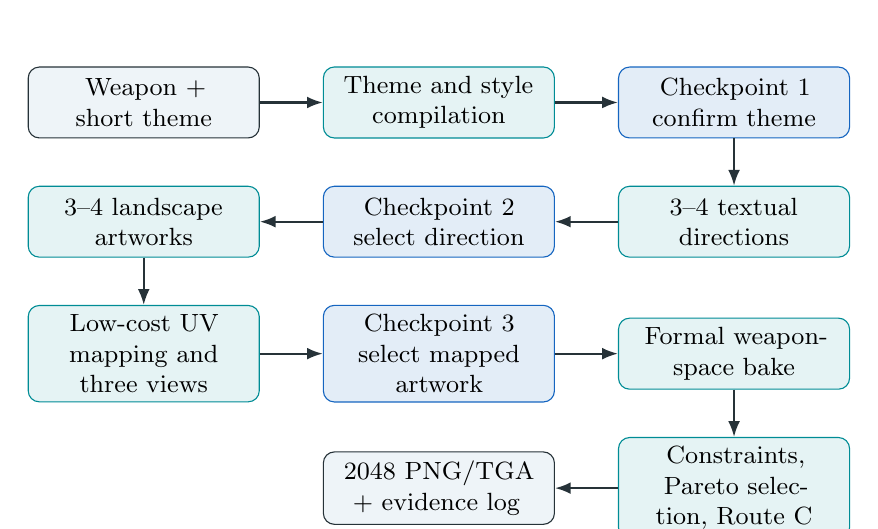
\begin{tikzpicture}[
    node distance=6mm and 8mm,
    box/.style={draw=skinsmithdark, rounded corners, align=center, minimum height=9mm,
      text width=27mm, fill=skinsmithlight, font=\small},
    checkpoint/.style={box, fill=skinsmithblue!12, draw=skinsmithblue},
    process/.style={box, fill=skinsmithteal!10, draw=skinsmithteal},
    arrow/.style={-{Latex[length=2mm]}, thick, draw=skinsmithdark}
  ]
    \node[box] (input) {Weapon + short theme};
    \node[process, right=of input] (theme) {Theme and style compilation};
    \node[checkpoint, right=of theme] (c1) {Checkpoint 1\\confirm theme};
    \node[process, below=of c1] (dirs) {3--4 textual directions};
    \node[checkpoint, left=of dirs] (c2) {Checkpoint 2\\select direction};
    \node[process, left=of c2] (art) {3--4 landscape artworks};
    \node[process, below=of art] (preview) {Low-cost UV mapping and three views};
    \node[checkpoint, right=of preview] (c3) {Checkpoint 3\\select mapped artwork};
    \node[process, right=of c3] (formal) {Formal weapon-space bake};
    \node[process, below=of formal] (eval) {Constraints, Pareto selection, Route C};
    \node[box, left=of eval] (export) {2048 PNG/TGA + evidence log};

    \draw[arrow] (input) -- (theme);
    \draw[arrow] (theme) -- (c1);
    \draw[arrow] (c1) -- (dirs);
    \draw[arrow] (dirs) -- (c2);
    \draw[arrow] (c2) -- (art);
    \draw[arrow] (art) -- (preview);
    \draw[arrow] (preview) -- (c3);
    \draw[arrow] (c3) -- (formal);
    \draw[arrow] (formal) -- (eval);
    \draw[arrow] (eval) -- (export);
  \end{tikzpicture}
  \caption{The \skinsmith\ workflow. The three blue nodes are blocking human
  checkpoints; formal processing cannot begin before a mapped artwork is selected.}
  \label{fig:architecture}
\end{figure}

\subsection{Agent state and human checkpoints}

An \texttt{AgentRunRequest} contains the asset identifier, a short theme or free
brief, an optional broad style family, the candidate count, and explicit budgets
for image calls, retries, and refinement rounds. The persisted state follows:

\begin{align*}
\texttt{created} &\rightarrow \texttt{planning}
\rightarrow \texttt{awaiting\_theme}
\rightarrow \texttt{awaiting\_direction}\\
&\rightarrow \texttt{awaiting\_artwork}
\rightarrow \texttt{executing}
\rightarrow \texttt{completed}.
\end{align*}

At the first checkpoint, a \texttt{ThemeCompiler} expands a compact keyword into a
validated \texttt{ThemePack}. The pack contains the concept, palette, primary and
supporting elements, environmental and material cues, atmosphere, component
story, evaluation criteria, and prohibited content. The user may confirm or edit
this interpretation. A \texttt{StyleCompiler} then produces three or four
materially different textual directions for the confirmed theme and selected
weapon. At the second checkpoint, the user chooses one direction.

The selected direction generates three or four dense landscape master artworks.
Each is validated for resolution, tonal and colour variation, local detail
density, and forbidden content. It is then passed through a low-cost mapping stage
using the target adapter. The original image and the left, right, and top views are
treated as one indivisible candidate card. The third checkpoint asks the user to
select one card. This design prevents a visually attractive source from being
chosen without seeing how it behaves on the asset.

The selected source path and hash become part of a frozen design contract. Formal
processing reuses that exact file; it does not regenerate an approximation after
selection. Every transition, tool action, budget change, retry, and stop reason is
written to persisted state so a failed or interrupted run can resume from the last
valid checkpoint.

\subsection{Asset adapter}

Each target is represented by a versioned \texttt{GameAssetAdapter}. The adapter
binds:

\begin{itemize}
  \item the mesh path, version, and SHA-256 hash;
  \item the authoritative UV source and UV address mode;
  \item canonical longitudinal and up axes;
  \item semantic regions and creative anchors;
  \item paintable-area rules;
  \item fixed cameras;
  \item texture size and export format.
\end{itemize}

This boundary is important because mesh geometry, UV charts, and material behavior
cannot be assumed to transfer between weapons. The accepted AK-47 adapter uses the
new CS2 geometry, a 2048 by 2048 RGB texture, fixed left/right/top cameras, and a
24-bit TGA Custom Paint export. The M4A4 case supplies a different mesh hash, axes,
UV topology, and seam calibration while reusing the core algorithms.

\subsection{Mesh-derived geometry maps}

Let a mesh triangle have three-dimensional vertices
$\mathbf{p}_0,\mathbf{p}_1,\mathbf{p}_2$, vertex normals
$\mathbf{n}_0,\mathbf{n}_1,\mathbf{n}_2$, and UV coordinates
$\mathbf{u}_0,\mathbf{u}_1,\mathbf{u}_2$. For every covered atlas pixel
$\mathbf{u}$, barycentric coordinates $(\lambda_0,\lambda_1,\lambda_2)$ are
computed in UV space. The corresponding position and normal are

\begin{align}
  \mathbf{p}(\mathbf{u}) &=
  \lambda_0\mathbf{p}_0+\lambda_1\mathbf{p}_1+\lambda_2\mathbf{p}_2,\\
  \tilde{\mathbf{n}}(\mathbf{u}) &=
  \lambda_0\mathbf{n}_0+\lambda_1\mathbf{n}_1+\lambda_2\mathbf{n}_2,\\
  \mathbf{n}(\mathbf{u}) &= \frac{\tilde{\mathbf{n}}(\mathbf{u})}
  {\lVert\tilde{\mathbf{n}}(\mathbf{u})\rVert_2}.
\end{align}

The mesh is transformed into a canonical frame whose $x$ axis follows the weapon
length, $y$ is up, and $z$ distinguishes the two sides. Positions are normalized
to the asset bounds. Rasterizing all UV triangles produces a position map, a
normal map, a valid-pixel mask, and a face-index map. These maps connect continuous
weapon-space composition to the existing fragmented atlas.

\subsection{Route A: tileable-pattern baseline}

\routeA\ generates a square, dense, crop-tolerant pattern. Its opposite image
borders are repaired using periodic-plus-smooth decomposition
\citep{moisan2011periodic}. The repaired square is then sampled through the
original UVs and rendered on the weapon. This route is deliberately generic: it
is expected to tolerate arbitrary crops, but it has no explicit whole-weapon
hierarchy.

Two seam concepts are recorded. The square-border error measures differences
between opposite image edges. The asset-seam error instead evaluates pairs of UV
edges that correspond to the same welded three-dimensional edge. Passing the
first measure does not imply passing the second.

\subsection{Route B: weapon-space composition and UV bake}

\routeB\ uses one selected landscape master artwork. The source is fitted to
continuous left, right, and top canvases in canonical weapon coordinates. The
source must be dense and edge-to-edge, with several medium or small thematic
clusters, because a single dominant subject or large empty region is unlikely to
survive the narrow silhouette and UV fragmentation.

For each valid UV pixel, the canonical position determines the sampling coordinate
on the side and top canvases. Surface normals blend the projections:

\begin{align}
  w_s &= |n_z|^p,\qquad w_t = \max(n_y,0)^p,\\
  \mathbf{c}(\mathbf{u}) &=
  \frac{w_s\mathbf{c}_s(\mathbf{p})+w_t\mathbf{c}_t(\mathbf{p})}
  {w_s+w_t+\epsilon},
\end{align}

where $p=4$ in the accepted configuration. $\mathbf{c}_s$ is sampled from the
appropriate left or right canvas according to surface orientation, while
$\mathbf{c}_t$ is sampled from the top canvas. This soft blend avoids an abrupt
switch between charts selected solely by the largest normal component.

\begin{figure}[t]
  \centering
  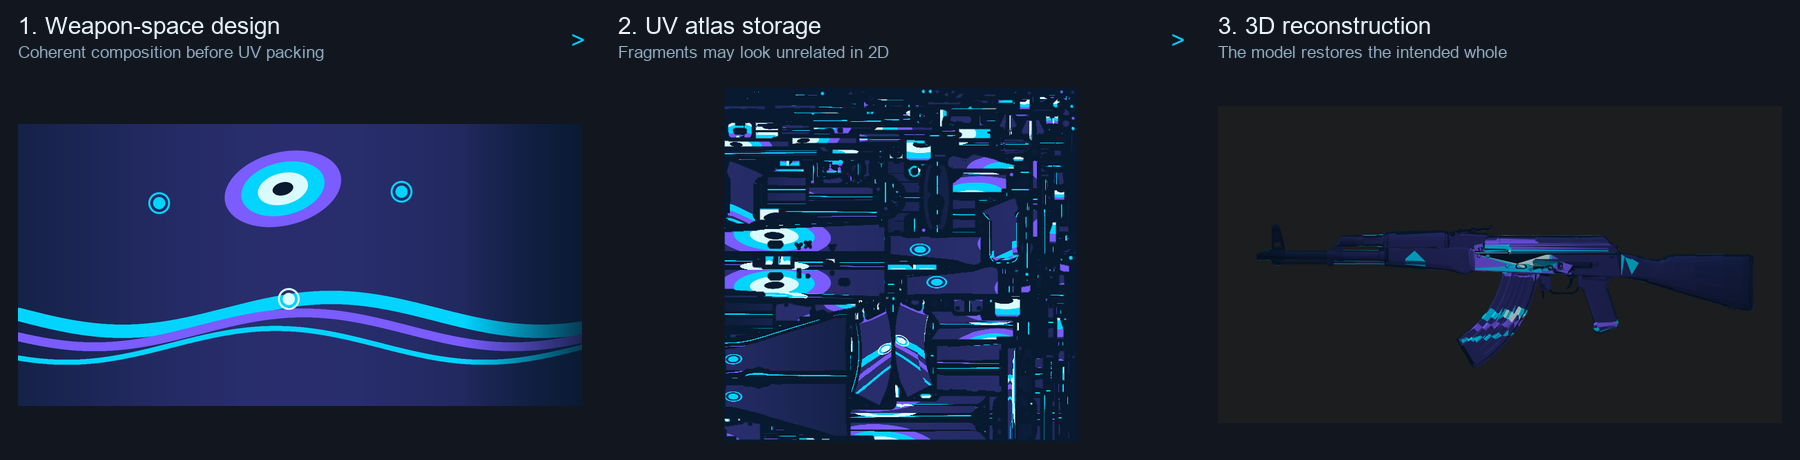
\includegraphics[width=\textwidth]{weapon_space_concept.png}
  \caption{The central Route B idea: compose in continuous weapon space, store
  fragments in the authoritative UV atlas, and judge coherence after
  reconstruction. The flat atlas is not expected to read as a conventional
  illustration.}
  \label{fig:weapon-space}
\end{figure}

\subsection{True asset-seam metric and correction}

OBJ files often duplicate vertices at UV boundaries. The method first welds
coordinate-identical geometric vertices, identifies mesh edges shared by adjacent
faces, and records pairs whose UV coordinates differ. These pairs form the true
asset-seam graph.

For $N$ paired samples with RGB colours $\mathbf{a}_i,\mathbf{b}_i$ and local
gradients $\mathbf{g}^{a}_i,\mathbf{g}^{b}_i$, the colour and gradient terms are

\begin{align}
  E_c &= \frac{1}{N}\sum_{i=1}^{N}
  \frac{\lVert\mathbf{a}_i-\mathbf{b}_i\rVert_1}{3\cdot255},\\
  E_g &= \frac{1}{N}\sum_{i=1}^{N}
  \frac{\lVert\mathbf{g}^{a}_i-\mathbf{g}^{b}_i\rVert_1}{3\cdot255}.
\end{align}

The implementation combines these normalized terms into $\assetseam$ using the
locked project weights. The principal hard requirement is
$\assetseam\leq0.01$.

An edge-safety correction blends a narrow region around UV-island boundaries
toward a stable base colour. Wider regions generally reduce seam error but can
erase visible detail. Candidate widths are therefore evaluated against both the
seam threshold and a minimum multi-view retention of 95\% relative to the
uncorrected texture.

\subsection{Rendering and evaluation}

The software renderer loads textured OBJ geometry, triangulates polygon faces,
interpolates UV coordinates barycentrically, samples the texture bilinearly, and
uses a z-buffer with fixed orthographic left, right, and top cameras. Lighting and
cameras are deterministic so candidates are compared under the same conditions.

Texture-level evidence includes contrast, saturation, detail, paintable coverage,
and square-border periodicity. The multi-view score combines foreground coverage,
contrast, saturation, visible detail, and luminance consistency across the three
views. The project also records mapped-element readability, defined as

\begin{equation}
  S_{\mathrm{read}} =
  0.25S_{\mathrm{source}}+
  0.50S_{\mathrm{left}}+
  0.15S_{\mathrm{right}}+
  0.10S_{\mathrm{top}}.
\end{equation}

This weighting reflects the principal inspection view in the case study. It is
recommendation-only and cannot override the user's artwork selection.

\subsection{Constraint-first selection}

For a candidate $x$, each hard constraint $j$ has a non-negative violation
$v_j(x)$. A candidate is feasible only if

\[
  V(x)=\sum_j v_j(x)=0.
\]

Feasible candidates are compared using Pareto dominance over the locked
objectives. If several candidates remain non-dominated, a deterministic priority
order selects the operating point. A conventional normalized weighted score is
retained only as an ablation baseline. This policy prevents a strong visual score
from compensating for a deployment failure.

\subsection{Route C: bounded local correction}

\routeC\ begins from the selected \routeB\ texture. Rendered component visibility
masks identify a component whose detail level deviates from its target. The Agent
creates exactly two correction candidates at fixed intensities. Changes are
restricted to that component plus a transition halo, and the number of changed
pixels outside the allowed region must be zero.

Each correction must retain all \routeB\ hard constraints. Let $S_B$ be the locked
score of the original and $S_C$ the best feasible correction. The correction is
accepted only when

\[
  S_C-S_B\geq0.01.
\]

Otherwise the final result is the unchanged \routeB\ texture. The method therefore
tests diagnosis and action without assuming that automatic refinement is
monotonic.

\subsection{Generation backends and evidence}

The generator interface supports a deterministic procedural baseline, a local
SD-Turbo model, and provider-backed image generation. SD-Turbo is pinned to
revision \path{b261bac6fd2cf515557d5d0707481eafa0485ec2} at 512 pixels, two
inference steps, and guidance scale zero. The accepted creative run used
\texttt{gemini-3.1-flash-lite} for structured planning and
\texttt{gemini-3.1-flash-image} for 1K landscape source images.

Every formal run preserves the request, prompts, provider and model identifiers,
seeds where applicable, redacted traces, source hashes, validation, mapped views,
UV outputs, metrics, decisions, budgets, retries, runtime, and checkpoints. API
keys are read from environment variables and are not written to run evidence.

\section{Experimental Design}
\label{sec:experiments}

\subsection{Evidence protocol}

Experiments were executed through repository scripts and preserved as immutable
run directories. Report tables were extracted from machine-readable JSON and CSV
records rather than copied from console output. Formal A/B/C evidence is kept
separate from earlier technical smokes and from the edge-width sub-ablation. This
separation is necessary because the candidate sources and experimental questions
differ.

The principal asset is an AK-47 mesh with 26,133 triangles, 21,548 UV coordinates,
928 UV islands, and 4,999 welded-topology seam pairs. The accepted texture size is
2048 by 2048 RGB for final export. Formal comparison runs use 512-pixel working
textures for controlled evaluation and share the target mesh, cameras, metrics,
palette, candidate count, and base seeds.

\subsection{Formal A/B/C comparison}

The formal experiment contains four paired candidates with seeds 20260716 to
20260719:

\begin{description}
  \item[\routeA] a generic pattern-first square source with periodic repair;
  \item[\routeB] a whole-weapon composition created in continuous weapon space,
  baked through OBJ-derived geometry maps, and corrected at UV edges;
  \item[\routeC] the corresponding \routeB\ result plus one diagnosis and two local
  correction attempts, subject to the 0.01 improvement gate.
\end{description}

\routeA\ and \routeB\ intentionally use different route-specific generation logic.
The comparison asks whether the weapon-aware representation produces better
mapped behavior, not whether identical pixels change after a single processing
operation. Within each route, the target, seed schedule, resolution, cameras, and
evaluation remain fixed.

For paired differences, the report gives the mean, median, standard deviation, win
rate, and bootstrap 95\% confidence interval. With only four pairs, these intervals
describe the observed candidate set and should not be read as population-level
proof across arbitrary themes or weapons.

\subsection{Seam-correction and selection-policy sub-ablations}

The seam-correction table compares each formal \routeB\ texture immediately before
and after the locked correction. This isolates the effect of the seam operation
without changing source content.

A separate edge-width sweep uses one unchanged earlier technical composition and
tests widths 0, 2, 4, 8, 12, 16, and 24 pixels. The hard conditions are
$\assetseam\leq0.01$ and multi-view retention of at least 95\%. The same candidate
pool is ranked by:

\begin{enumerate}
  \item feasibility, Pareto dominance, and deterministic objective order; and
  \item an equal 50/50 normalized weighted score.
\end{enumerate}

This sweep supports claims about operating-point and policy behavior. It is not
used to claim that the earlier artwork is visually superior to the final
generated candidates.

\subsection{Three-checkpoint live case}

The interaction case begins with a dragon theme and the AK-47 adapter. The Agent
produces four directions; the user selects \emph{Treasured Relic}. Four landscape
artwork variations are generated and mapped at low cost. One failed source
attempt, containing large empty regions and isolated clusters, is rejected and
regenerated locally rather than restarting the complete run. The user selects
\texttt{artwork\_04} after viewing the source with its left, right, and top
previews. Formal 2048 processing then reuses the selected source exactly.

This case is not merged with the procedural formal A/B/C pool. Its purpose is to
test the complete human-Agent interaction, real image-generation backend,
checkpoint persistence, candidate-local retry, and final export contract.

\subsection{Adapter transfer case}

The M4A4 case reuses the same theme assets and core algorithms with zero additional
image-generation calls. Only the adapter, official mesh hash, canonical axes, UV
topology, and seam calibration change. The M4A4 mesh contains 45,422 triangles,
39,881 UV coordinates, 1,747 UV islands, and 11,341 seam pairs. The test asks
whether the pipeline executes and where the AK-47 thresholds cease to transfer.

\subsection{Evaluation criteria}

The report uses the following primary measures:

\begin{itemize}
  \item asset-seam error $\assetseam$ (lower is better);
  \item multi-view score $\multiview$ (higher is better);
  \item multi-view retention relative to the uncorrected candidate;
  \item locked Agent score for Route C accept/rollback decisions;
  \item changed-pixel fraction and changed pixels outside the target halo;
  \item successful completion of the three blocking human checkpoints;
  \item final texture resolution, colour mode, export identity, and file hash.
\end{itemize}

Automatic readability is reported only for explanation. It is not a substitute
for a human preference study, and no claim is made that it measures general
aesthetic quality.

\subsection{Implementation and reproducibility}

The implementation uses Python 3.13, NumPy, Pillow, OpenCV, SciPy, PyTorch,
Transformers, Diffusers, and Streamlit. The local diffusion acceptance used an
NVIDIA RTX 4060 Laptop GPU with 8 GB VRAM. The repository contains a deterministic
procedural backend, a pinned SD-Turbo backend, provider adapters, the Agent
runtime, command-line scripts, and a thin Streamlit client. At the report freeze,
100 unit tests, Python byte-code compilation, configuration parsing, and headless
Streamlit startup had passed.

The public repository is \url{\repositoryurl}. Valve geometry, model weights, and
API keys are intentionally excluded. Setup documentation explains how authorized
users obtain external assets and configure local credentials.

\section{Results}
\label{sec:results}

\subsection{RQ1: weapon-space composition}

\Cref{tab:formal-candidates} reports the four paired candidates. \routeB\ reduces
asset-seam error from 0.2438--0.2967 to below 0.0008 for every pair. It also
improves the multi-view score for every pair, despite a modest reduction in the
texture-only score. Candidate 04 is selected within \routeB.

\begin{table}[t]
  \centering
  \caption{Formal paired A/B results. Lower asset-seam error is better; higher
  texture and multi-view scores are better.}
  \label{tab:formal-candidates}
  \small
  \begin{tabular}{llrrrr}
    \toprule
    Route & Candidate & Asset seam & Multi-view & Texture & Selected\\
    \midrule
    A & 01 & 0.286821 & 0.752696 & 0.761178 & No\\
    A & 02 & 0.252571 & 0.792474 & 0.779769 & Yes\\
    A & 03 & 0.243767 & 0.767358 & 0.770474 & No\\
    A & 04 & 0.296737 & 0.763398 & 0.776778 & No\\
    \midrule
    B & 01 & 0.000473 & 0.819614 & 0.765960 & No\\
    B & 02 & 0.000635 & 0.818653 & 0.749159 & No\\
    B & 03 & 0.000617 & 0.833842 & 0.755199 & No\\
    B & 04 & 0.000796 & 0.844312 & 0.751902 & Yes\\
    \bottomrule
  \end{tabular}
\end{table}

The paired summary in \cref{tab:paired-summary} shows a mean asset-seam
improvement of 0.26934 and a mean multi-view improvement of 0.06012. The win rate
is 100\% on both measures. The bootstrap intervals remain above zero for the four
observed pairs.

\begin{table}[t]
  \centering
  \caption{Paired Route B minus Route A summary ($n=4$).}
  \label{tab:paired-summary}
  \small
  \begin{tabular}{lrrrrr}
    \toprule
    Metric & Mean & Median & Std. & Win rate & Bootstrap 95\% CI\\
    \midrule
    Asset-seam improvement & 0.269344 & 0.269142 & 0.022281 & 100\% &
    [0.247543, 0.291145]\\
    Multi-view improvement & 0.060124 & 0.066701 & 0.020440 & 100\% &
    [0.036363, 0.077307]\\
    \bottomrule
  \end{tabular}
\end{table}

\begin{figure}[t]
  \centering
  \begin{subfigure}[t]{0.49\textwidth}
    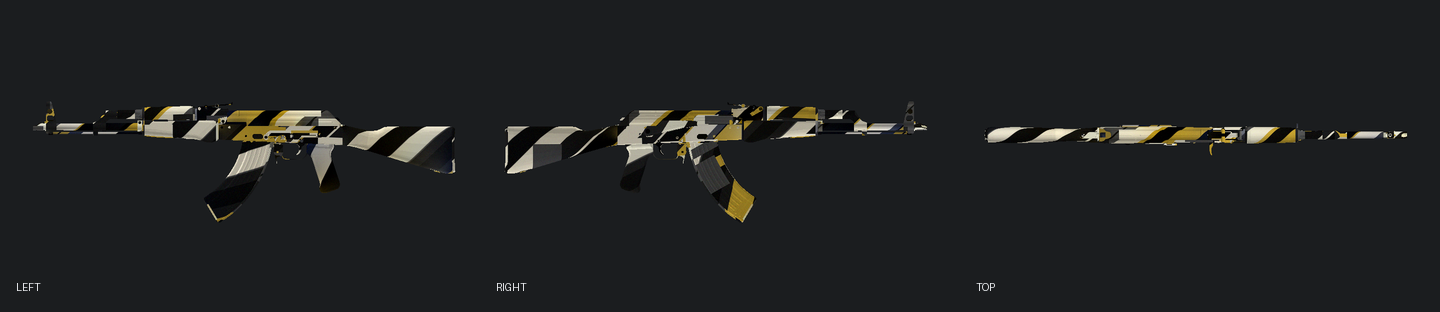
\includegraphics[width=\textwidth]{formal_route_a_candidate04.png}
    \caption{Route A candidate 04}
  \end{subfigure}
  \hfill
  \begin{subfigure}[t]{0.49\textwidth}
    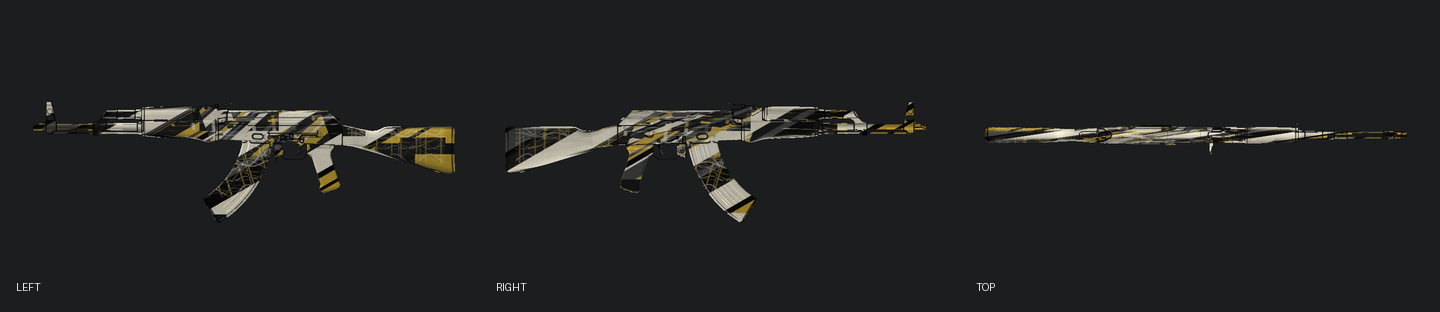
\includegraphics[width=\textwidth]{formal_route_b_candidate04.png}
    \caption{Route B candidate 04}
  \end{subfigure}
  \caption{Mapped left, right, and top views for the same candidate index in the
  formal experiment. Route A behaves as an all-over pattern; Route B reconstructs
  a continuous composition after UV fragmentation.}
  \label{fig:formal-ab}
\end{figure}

The formal seam-correction operation reduces the mean \routeB\ seam error by
99.62\%. Before correction, the four values range from 0.14986 to 0.17639; after
correction, all are below 0.0008 and pass the 0.01 threshold. This establishes that
the low final seam error is not merely inherited from the source artwork.

These results answer RQ1 positively for the tested AK-47 candidates. The conclusion
is bounded to this asset, theme family, renderer, and four-pair sample.

\subsection{RQ2: failures exposed by mapped evaluation}

The live dragon case provides direct examples of why source images are
insufficient. One attempted artwork passed technical image checks but was rejected
because its subjects formed isolated clusters around large dark regions. Such a
composition is fragile under cropping and UV fragmentation. After a local retry,
all four candidate sources were mapped before selection.

\begin{figure}[t]
  \centering
  \begin{subfigure}[t]{0.98\textwidth}
    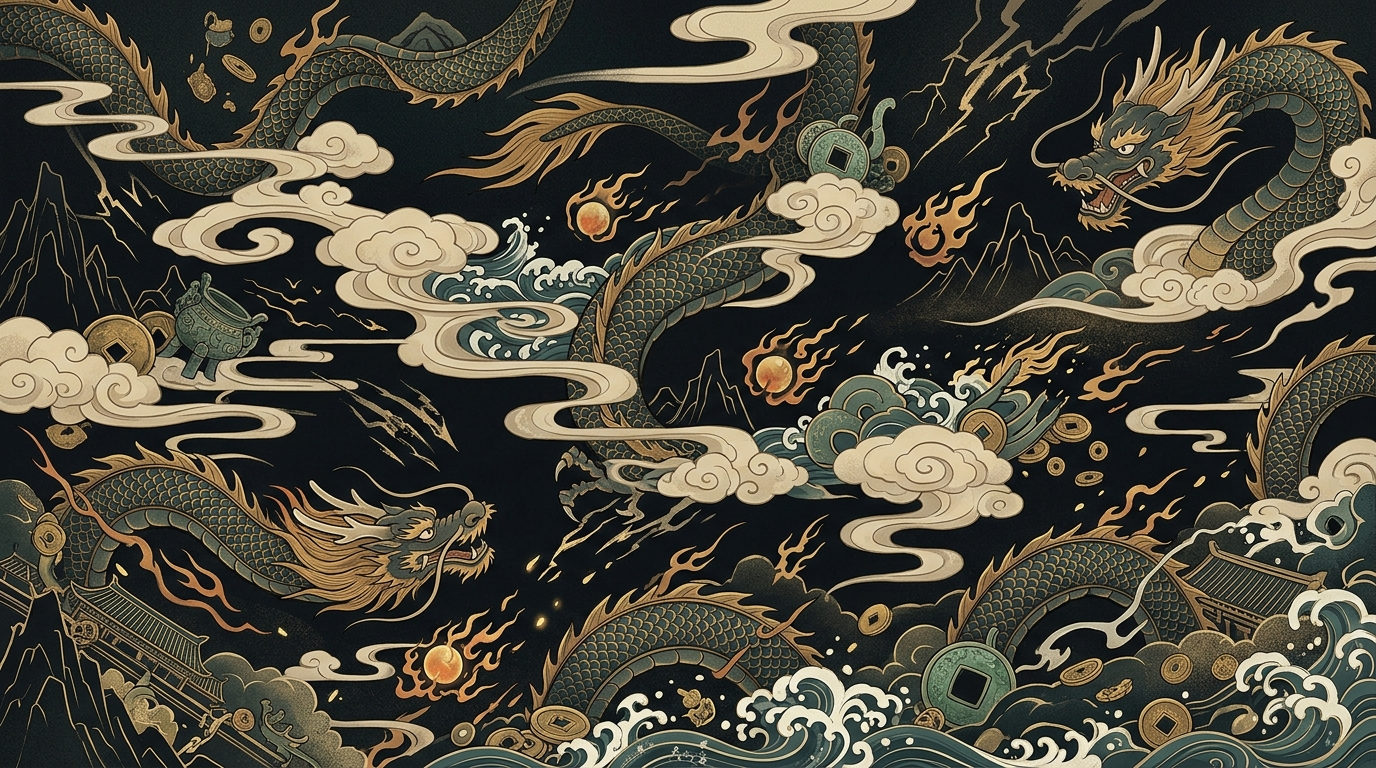
\includegraphics[width=\textwidth]{selected_master_artwork.png}
    \caption{Human-selected landscape source artwork}
  \end{subfigure}
  \vspace{2mm}
  \begin{subfigure}[t]{0.98\textwidth}
    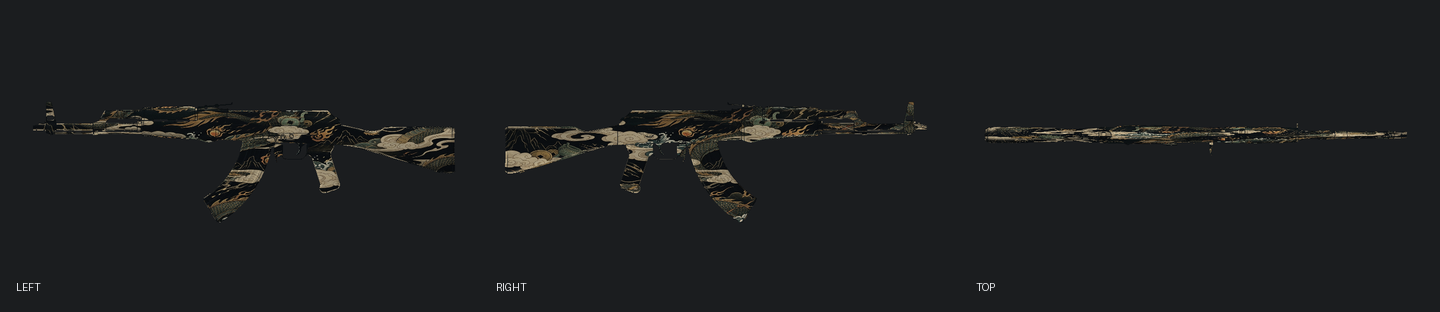
\includegraphics[width=\textwidth]{dragon_route_b_multiview.png}
    \caption{Formal Route B left, right, and top reconstruction}
  \end{subfigure}
  \caption{The selected source and its mapped result are related but not
  interchangeable evidence. The narrow top view and UV fragmentation remove or
  compress details that appear clear in the source.}
  \label{fig:dragon-selected}
\end{figure}

For the selected source, automatic review reports source fulfillment 0.9386, left
readability 0.6016, right readability 0.6016, and top readability 0.3993. Only
eight of sixteen planned elements exceed the visibility threshold. The top view
is the weakest because of its narrow projected area, while the source score is
much higher. This difference is the central observation for RQ2: mapping reveals
loss of readable elements, view imbalance, component-specific cropping, and
seam behavior that cannot be inferred reliably from the rectangular artwork.

The route comparison in \cref{fig:dragon-routes} illustrates a second failure
mode. The generated \routeA\ image has a high multi-view score of 0.8952, but its
asset-seam error is 0.1822 and it fails the deployment constraint. A strong
aggregate visual score is therefore not evidence of a technically valid texture.

\begin{figure}[t]
  \centering
  \begin{subfigure}[t]{0.49\textwidth}
    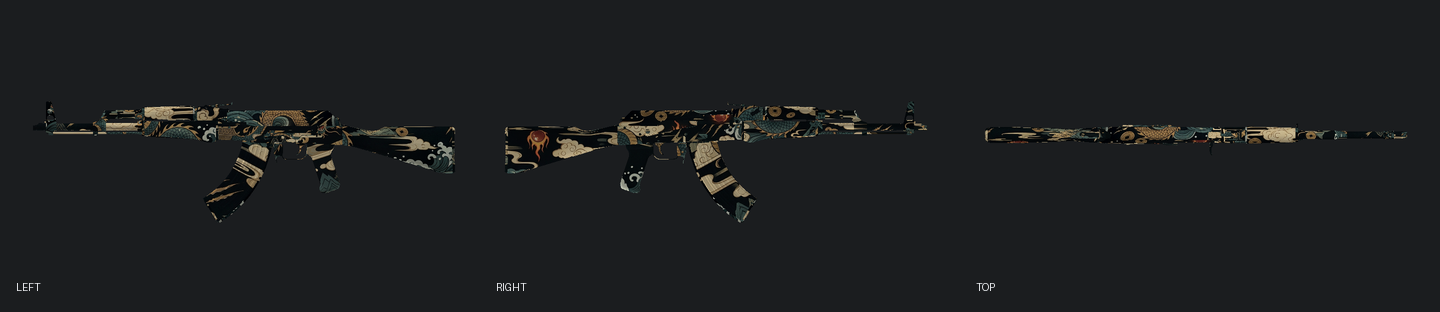
\includegraphics[width=\textwidth]{dragon_route_a_multiview.png}
    \caption{Route A: strong visible activity, invalid asset seam}
  \end{subfigure}
  \hfill
  \begin{subfigure}[t]{0.49\textwidth}
    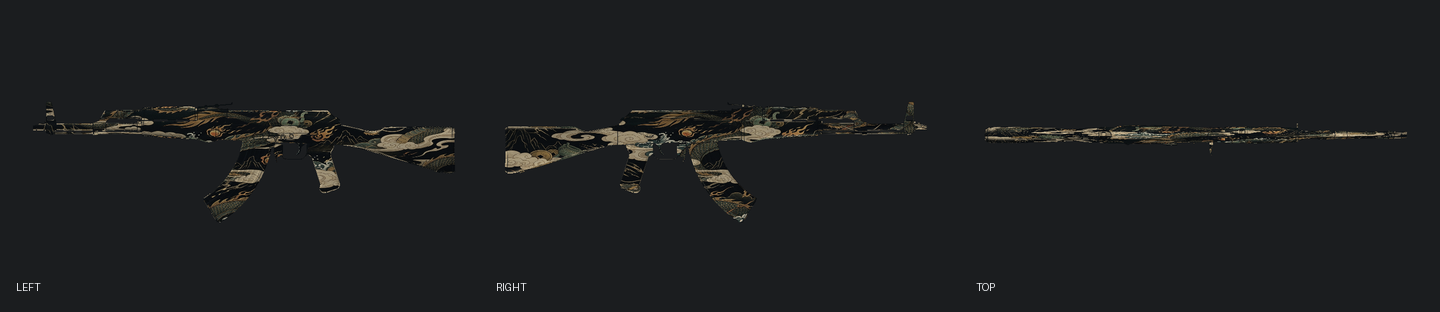
\includegraphics[width=\textwidth]{dragon_route_b_multiview.png}
    \caption{Route B: valid seam and continuous mapped composition}
  \end{subfigure}
  \caption{The final live case separates visual activity from deployment
  feasibility.}
  \label{fig:dragon-routes}
\end{figure}

\subsection{RQ3: constrained selection and rollback}

\Cref{fig:edge-sweep} shows the expected trade-off in the independent edge-width
study. Increasing the safety width reduces seam error but gradually removes
multi-view detail. Widths 8, 12, and 16 are feasible and Pareto-optimal. Width 24
has a lower seam error but falls below 95\% retention.

\begin{figure}[t]
  \centering
  \begin{tikzpicture}
    \begin{axis}[
      width=0.92\textwidth,
      height=62mm,
      xlabel={Edge-safety width (pixels)},
      ylabel={Score},
      xmin=0,xmax=24,
      ymin=0,ymax=1.02,
      grid=both,
      legend style={at={(0.5,-0.22)},anchor=north,legend columns=3},
      mark size=2.3pt
    ]
      \addplot+[thick,mark=*,skinsmithblue]
        table[x=edge_safe_pixels,y=asset_seam_error,col sep=comma]
        {data/table_edge_safety_sweep.csv};
      \addlegendentry{Asset-seam error}
      \addplot+[thick,mark=square*,skinsmithteal]
        table[x=edge_safe_pixels,y=multi_view_score,col sep=comma]
        {data/table_edge_safety_sweep.csv};
      \addlegendentry{Multi-view score}
      \addplot+[thick,mark=triangle*,orange]
        table[x=edge_safe_pixels,y=multi_view_retention,col sep=comma]
        {data/table_edge_safety_sweep.csv};
      \addlegendentry{Multi-view retention}
      \addplot[red,dashed,domain=0:24] {0.01};
      \addplot[gray,dashed,domain=0:24] {0.95};
    \end{axis}
  \end{tikzpicture}
  \caption{Independent edge-width sweep. Width 8 is the selected feasible
  operating point. The two dashed lines show the seam and retention thresholds.}
  \label{fig:edge-sweep}
\end{figure}

The policy ablation is decisive. Equal weighted ranking selects width 4 because it
retains a multi-view score of 0.70324, but its seam error is 0.01660 and therefore
invalid. Constraint-first/Pareto selection chooses width 8, with seam error
0.00552 and multi-view score 0.69697. The weighted approach hides a hard violation
behind a small visual gain.

All four formal \routeC\ cases execute two local corrections. The selected
attempts change 2.33--2.93\% of atlas pixels and change zero pixels outside the
target component plus halo. Their best locked-score changes are -0.00110,
-0.00110, -0.00082, and -0.00088, all below the required +0.01. Consequently,
every final C result equals B. In the live dragon case, the best correction changes
the score by -0.02196 and is also rolled back.

RQ3 is therefore supported in two ways: feasibility-first selection rejects a
candidate preferred by a soft score, and the acceptance gate prevents a lower
quality correction from replacing its baseline. The result does not show that
refinement improves quality; it shows that attempted refinement is bounded.

\subsection{RQ4: three-checkpoint collaboration}

The live Agent completes the intended interaction:

\begin{enumerate}
  \item the theme is expanded into dragons, clouds, waves, treasure, flaming
  pearls, mountains, lightning, mist, jade, and architectural fragments;
  \item four directions are presented, and \emph{Treasured Relic} is selected;
  \item four artworks are generated and mapped, and \texttt{artwork\_04} is
  selected from its source-plus-three-view card.
\end{enumerate}

The run uses six image calls, one local retry, and one refinement round. It ends in
the \texttt{completed} state and exports a 2048 by 2048 RGB PNG and TGA with
identical decoded pixels. The final \routeB\ result has asset-seam error 0.000778,
multi-view score 0.816620, and total score 0.829123. The source hash and final TGA
hash are preserved.

This case answers RQ4 at the level of functional workflow: a user can begin from a
compact theme, make three distinct decisions, and receive a formally processed
texture without authoring a production prompt. It does not constitute a usability
study; no completion-time or user-satisfaction comparison was conducted.

\subsection{RQ5: adapter-based portability}

The M4A4 adapter executes geometry mapping, continuous composition, UV baking,
seam measurement, rendering, and evaluation with no new image-generation call.
\Cref{fig:m4-transfer} confirms that the same conceptual pipeline reconstructs a
mapped texture on different geometry.

\begin{figure}[t]
  \centering
  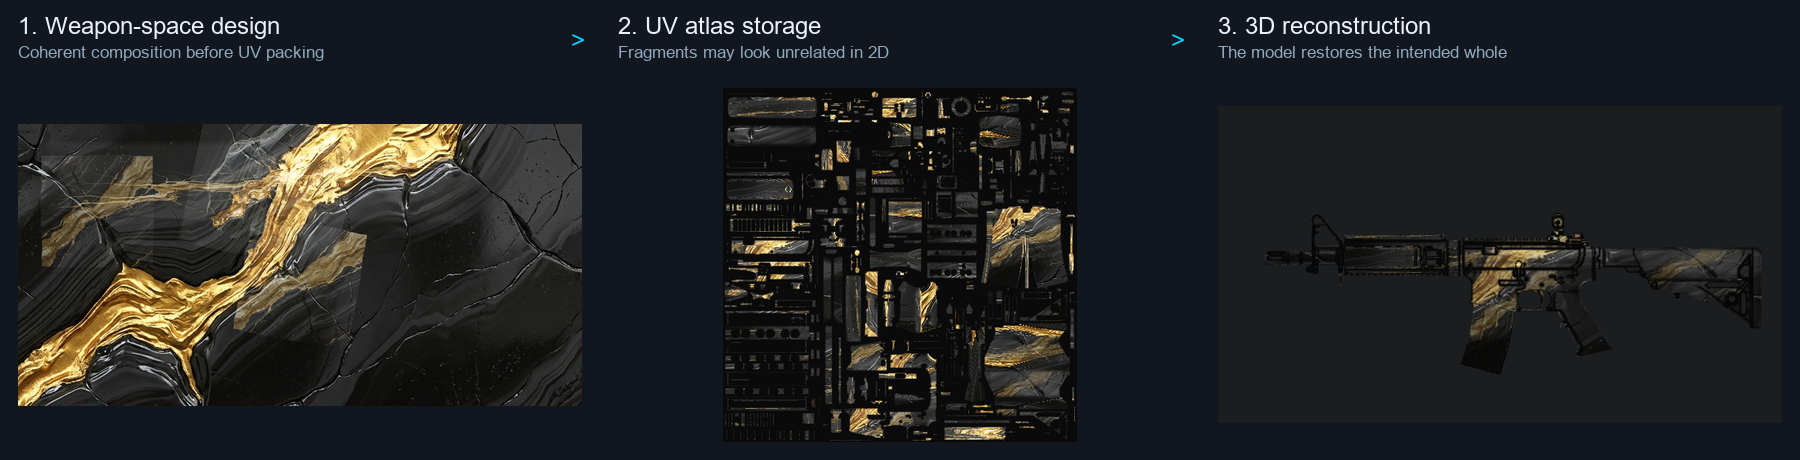
\includegraphics[width=\textwidth]{m4a4_transfer_concept.png}
  \caption{M4A4 adapter transfer. The core method is reused, but the denser UV
  topology requires different seam calibration.}
  \label{fig:m4-transfer}
\end{figure}

Transfer is only partial. The best joint candidate reaches seam error 0.00994 but
retains 94.02\% of the raw multi-view score, below the AK-47 threshold of 95\%.
The M4A4 contains 1,747 UV islands and 11,341 seam pairs, compared with 928 islands
and 4,999 pairs for the AK-47. More aggressive seam treatment improves continuity
but removes too much visible detail.

RQ5 is therefore answered by a boundary rather than a universal success:
planning, composition, bake, rendering, metrics, and logging transfer; mesh, UV,
axes, camera, material, and correction calibration remain adapter-specific.

\section{Discussion}
\label{sec:discussion}

\subsection{Interpretation of the findings}

The strongest result is not that \routeB\ produces a more attractive square
texture. Its flat atlas is often less legible than \routeA\ because it stores
pieces of a continuous composition. The relevant result is that the composition
reconstructs on the weapon while satisfying a true asset-seam constraint. This
changes the unit of evaluation from the generated rectangle to the mapped asset.

The paired experiment supports that representation choice for the tested AK-47
candidates. All four \routeB\ candidates improve both seam and multi-view
performance. The seam gain is expected in part because \routeB\ explicitly
contains an asset-edge operation, but the simultaneous multi-view gain is
important: continuity was not purchased by simply flattening all visible detail.
The separate before/after table further isolates the seam correction and shows
that the operation, rather than the generator alone, is responsible for the low
final error.

The live case complicates a simple ``higher score is better'' interpretation.
\routeA\ obtains a higher multi-view score than the selected \routeB\ texture, yet
fails the asset-seam threshold by a large margin. This is precisely the situation
in which feasibility must precede preference. The edge-width ablation reaches the
same conclusion under a fixed candidate pool: a small gain in multi-view score
causes the weighted policy to choose an invalid candidate.

The rollback results are also informative. None of the formal \routeC\ attempts
improves the locked score, and the live correction is distinctly worse. Reporting
these outcomes avoids presenting the Agent as an automatically self-improving
system. The contribution is narrower and more defensible: the Agent can identify a
target, produce local alternatives, prove locality, and decline to replace a
better baseline.

\subsection{Metric appraisal}

The evaluation stack deliberately contains several measures because no single
metric captures deployable visual quality. Asset-seam error has a clear technical
interpretation, but a very low value can be achieved by over-smoothing boundaries.
Multi-view retention protects against that failure, although it still summarizes
contrast, saturation, detail, coverage, and consistency rather than aesthetic
quality.

The component-detail balance metric failed on high-contrast weapon-space
candidates: several \routeB\ values collapsed to zero and made the locked Agent
score lower even when seam and multi-view performance improved. For this reason,
the component-balance and aggregate-score differences are not used as evidence
that \routeA\ is superior. They are retained as a documented metric limitation and
as motivation for reporting primary measures separately.

Mapped-element readability has a similar boundary. The selected artwork scores
highly at the source and substantially lower on the top view, which is useful
diagnostic information. However, it depends on model-based semantic judgments and
view weighting chosen for this case study. The human artwork decision remains
authoritative.

\subsection{Internal and external validity}

Several controls strengthen internal validity: fixed assets and cameras, shared
seed schedules within the formal comparison, exact source reuse after human
selection, machine-readable logs, isolated sub-ablations, and deterministic
rendering. The renderer, UV bake, seam metric, selection policy, and locality gate
also have regression tests.

The main threat is sample size. Four formal pairs are sufficient to expose
consistent behavior in the preserved candidate set but not to estimate performance
over the space of themes, generators, or weapons. Route-specific generation logic
also means the comparison evaluates two complete design strategies rather than a
single-factor image transformation. This is appropriate for the research question,
but the result should not be interpreted as a causal estimate of one isolated
algorithmic component.

External validity is limited by one complete weapon, one principal creative case,
one software renderer, and a small set of backends. The M4A4 result is useful
because it fails the joint threshold: it shows that adapter portability is not the
same as parameter portability. Broader claims would require several weapon
families, game material systems, viewing conditions, and users.

\subsection{Human-Agent interaction limitations}

The three checkpoints solve a structural problem: they separate interpretation,
creative direction, and mapped artwork. They also make disagreement recoverable.
A user can edit a theme before generation, reject an unwanted direction, or reject
an artwork after mapping without discarding the complete run.

The present study verifies this contract technically, but does not compare it with
a one-prompt baseline through a user study. Future work should measure task time,
number of revisions, perceived control, preference confidence, and the frequency
with which source-only and mapped choices disagree. Such a study would provide
stronger evidence for RQ4 beyond successful execution.

\subsection{Material-channel and engine-validation boundary}

The implemented output is a base-colour texture for the Custom Paint Job
workflow. It does not generate aligned normal, roughness, metallic, height, or
displacement maps, and it should therefore not be described as a complete
physically based material authoring system. The current contribution concerns
semantic planning, colour-texture composition, UV-aware baking, mapped-view
evaluation, and constrained selection.

CS2 Workbench captures provide important deployment evidence, but their lighting
and reflectance are produced by the engine and finish configuration. They do not
demonstrate model-generated surface relief or material response. The known-good
calibration case verifies the UV orientation and import contract, while the
black-and-gold marble case verifies coherent in-engine colour-texture deployment.
These cases are kept distinct from the accepted live dragon Agent run, whose
final TGA still requires a fixed left/right/top Workbench capture for the strongest
end-to-end visual record.

The most direct technical extension is a multi-channel material pipeline that
generates spatially aligned base-colour, normal, roughness, and metallic maps,
checks cross-channel consistency, and validates the result under fixed engine
lighting. This would require material-aware metrics and export adapters in
addition to the present UV and colour-texture checks.

\subsection{Project management and methodological evolution}

The registered topic, \emph{Latent Vision $\rightarrow$ Image Generation}, was
intentionally broad and emphasized image-to-image workflows, diffusion models,
conditioning, and creative visual outputs. Supervisor guidance later superseded
that original scope: given the remaining delivery window, completing the technical
development of an image-processing Agent was considered sufficient, and the Agent
did not need to preserve the original Latent Vision framing. The team therefore
treated SkinSmith as a focused implementation of the approved image-processing
Agent direction rather than as an attempt to cover every objective in the original
topic description.

Work then progressed through dated milestones: deterministic generation and seam
repair; real OBJ rendering; local diffusion; UV and seam diagnostics; weapon-space
composition; formal A/B/C experiments; provider-backed generation; the reusable
Agent runtime; the three-checkpoint client; and academic production.

Several changes were driven by failed evidence rather than by the original plan.
Direct border blending was removed after it produced a visible mirrored frame.
An early mask-aware route was retained as negative evidence because it changed
component appearance without creating a coherent whole-weapon composition.
Per-component dragon generation was abandoned after it produced semantically wrong
source parts and framed panels. A legacy UV assumption was rejected after
deployment mismatch. These corrections delayed the interface, but reduced the risk
of polishing a workflow whose asset contract was wrong.

The group used five connected work packages with one integration lead. YUAN Ye
served as project lead and integration owner, defining the system architecture and
coordinating the shared Agent contract. CHEN Yuhong owned creative planning and
literature synthesis; Ben Tangjie owned generation-backend integration and
reproducibility; Wang Zhengye owned asset, UV, and rendering validation; and WANG
Lihui owned evaluation, experiment reporting, and submission quality control.
Each work package contributed method decisions, implementation or configuration,
experimental verification, and documentation to the final system. This structure
gave every member an assessable technical contribution while retaining one owner
for cross-module consistency.

\subsection{Responsible use, provenance, and rights}

The project uses generative models as experimental components. Structured theme
and style planning in the accepted live case used
\texttt{gemini-3.1-flash-lite}; source artwork used
\texttt{gemini-3.1-flash-image}; and SD-Turbo provided a pinned local baseline.
Prompts, model identifiers, validation traces, and source hashes are recorded.
Credentials are supplied through local environment variables and removed from
evidence.

The system is restricted to original themes and explicitly prohibits copied skins,
logos, brands, teams, protected characters, text, watermarks, and imitation of a
named living artist. Generated sources are reviewed before mapping. Valve geometry
is used only as an external case-study asset and is not redistributed in the
repository. The report does not claim ownership of Valve assets, affiliation with
Valve, or readiness for Steam Workshop publication.

These safeguards do not resolve every concern. The training data of external image
models are not controlled by this project, and automated filters can miss
similarity or embedded content. Any use beyond the academic prototype would
require model-licence review, independent rights checking, stronger moderation,
game-specific terms review, and a clear appeals process for rejected or disputed
content.

\subsection{Practical implications}

Three practical lessons follow from the study:

\begin{enumerate}
  \item A source image should not be approved before it is mapped. Candidate cards
  should bind the source to the views on which it will be judged.
  \item A deployment constraint should not be averaged into a general quality
  score. Feasibility and preference answer different questions.
  \item Agent refinement should have a budget and a rollback rule. In creative
  pipelines, a plausible correction can still remove valuable detail.
\end{enumerate}

These lessons extend beyond weapon skins to other assets whose appearance is
stored in fragmented atlases, including props, clothing, vehicle parts, and
product visualizations. The geometry and deployment adapters would change, but
the evidence and decision structure would remain relevant.

\section{Conclusion}
\label{sec:conclusion}

This project investigated how a compact visual theme can be converted into a
mapped, technically valid, and reproducible game-asset texture. The resulting
\skinsmith\ prototype combines three human checkpoints with asset-aware
generation, deterministic UV baking, multi-view evaluation, hard feasibility
rules, and one bounded refinement round.

For RQ1, the four-pair AK-47 experiment shows that composing in continuous
weapon space and baking into the existing atlas improves both true asset-seam and
multi-view performance relative to the tileable baseline in every observed pair.
For RQ2, mapped evaluation exposes view-specific loss, internal seam failure, and
the difference between an attractive source and a usable texture. For RQ3, the
selection-policy ablation and the Route C results show that hard constraints and
rollback prevent acceptance of infeasible or lower-scoring candidates. For RQ4,
the live run demonstrates a complete path from a short theme through theme,
direction, and mapped-artwork decisions to a 2048 PNG/TGA export. For RQ5, the
M4A4 case shows that the core pipeline transfers through an adapter, while UV
topology and correction parameters remain asset-specific.

The main conclusion is methodological: image generation should be treated as one
stage in an asset pipeline, not as the endpoint. A credible generative Agent must
show what happens after mapping, preserve the user's authority where metrics are
weak, distinguish feasibility from preference, and retain the evidence behind
acceptance and rollback.

The current system is deliberately limited to base-colour Custom Paint Job
textures. It does not generate normal, roughness, metallic, height, or displacement
channels; Workbench lighting must therefore not be interpreted as generated
surface detail. Before final submission, the highest-value evidence addition is a
fixed left/right/top Workbench capture of the exact accepted dragon TGA, together
with one screenshot of the import settings.

Future work should proceed in four stages. First, add spatially aligned normal,
roughness, and metallic generation with cross-channel and engine-side validation.
Second, automate fixed-camera Workbench or game-engine capture so that deployment
evidence is reproducible. Third, evaluate more weapon and non-weapon adapters and
learn asset-specific correction parameters. Fourth, improve perceptual measures
and conduct a user study of the three checkpoints, including task time, revision
count, perceived control, and disagreements between source-only and mapped
choices. These extensions would test generalisation without weakening the bounded
claims established here.


\clearpage
\bibliographystyle{plainnat}
\bibliography{references}

\clearpage
\appendix
\section{Reproducibility}
\label{app:reproducibility}

\subsection{Repository}

The project repository is:

\begin{center}
  \url{\repositoryurl}
\end{center}

External Valve assets, model weights, and API credentials are not included.
The repository setup guide describes how to obtain authorized geometry and
configure local dependencies.

\subsection{Core commands}

\begin{lstlisting}[basicstyle=\ttfamily\small,breaklines=true,frame=single]
.\.venv\Scripts\python.exe -m unittest discover -s tests -v
.\.venv\Scripts\python.exe -m compileall -q src scripts streamlit_app.py tests
.\.venv\Scripts\python.exe scripts\smoke_test.py
.\.venv\Scripts\python.exe scripts\real_model_smoke_test.py
.\.venv\Scripts\python.exe scripts\abc_ablation_formal.py
.\.venv\Scripts\python.exe scripts\build_report_ablation_tables.py
.\.venv\Scripts\python.exe -m streamlit run streamlit_app.py
\end{lstlisting}

The exact arguments for provider-backed runs and checkpoint resume are documented
in the repository because they depend on local credentials and preserved run
state.

\section{Evidence index}
\label{app:evidence}

\begin{table}[H]
  \centering
  \caption{Machine-readable evidence used in the report. Paths are relative to the
  repository root.}
  \small
  \begin{tabularx}{\textwidth}{p{35mm} X}
    \toprule
    Claim or artifact & Preserved evidence\\
    \midrule
    Formal A/B/C candidates &
    \path{runs/abc_ablation_true_weapon_space/ablation_log.json}\\
    Paired statistics &
    \path{runs/report_ready_ablation_tables/table_abc_paired_summary.csv}\\
    Formal seam correction &
    \path{runs/report_ready_ablation_tables/table_formal_b_seam_correction.csv}\\
    Edge-width sweep &
    \path{runs/report_ready_ablation_tables/table_edge_safety_sweep.csv}\\
    Selection-policy comparison &
    \path{runs/report_ready_ablation_tables/table_selection_policy_comparison.csv}\\
    Formal Route C attempts &
    \path{runs/report_ready_ablation_tables/table_route_c_attempts.csv}\\
    Three-checkpoint live case &
    \path{runs/agent_dragon_multicandidate_v1/agent_run_result.json}\\
    Artwork alternatives &
    \path{runs/agent_dragon_multicandidate_v1/artwork_candidates.json}\\
    Mapped readability &
    \path{runs/agent_dragon_multicandidate_v1/execution/mapped_element_readability.json}\\
    M4A4 transfer &
    \path{runs/m4a4_game_asset_adapter_transfer/transfer_final.json}\\
    \bottomrule
  \end{tabularx}
\end{table}

\section{Formal Route C attempts}

\begin{table}[H]
  \centering
  \caption{Best correction attempt for each formal Route B candidate. All
  modifications remain inside the target component and transition halo.}
  \small
  \begin{tabular}{lrrrr}
    \toprule
    Candidate & Changed fraction & Outside-halo pixels & Score change & Accepted\\
    \midrule
    01 & 0.028670 & 0 & -0.001097 & No\\
    02 & 0.029309 & 0 & -0.001095 & No\\
    03 & 0.023314 & 0 & -0.000816 & No\\
    04 & 0.027806 & 0 & -0.000880 & No\\
    \bottomrule
  \end{tabular}
\end{table}

\section{Milestone summary}

\begin{table}[H]
  \centering
  \caption{Development milestones and corrective decisions.}
  \small
  \begin{tabularx}{\textwidth}{p{25mm} p{38mm} X}
    \toprule
    Stage & Completed capability & Evidence-based adjustment\\
    \midrule
    Foundation & Procedural candidates, periodic repair, metrics, logs &
    Mirrored border blending was replaced after visual failure.\\
    Real asset loop & OBJ/UV rendering and fixed three-view evaluation &
    Flat texture quality was no longer treated as sufficient evidence.\\
    UV diagnosis & Welded seam graph, masks, asset binding &
    Incompatible legacy UV assumptions were rejected.\\
    Weapon-space route & Canonical frame, geometry maps, continuous composition &
    Mask-only remapping was retained as negative evidence and replaced.\\
    Formal evaluation & A/B/C, seam and policy sub-ablations, M4A4 transfer &
    Metrics with invalid behavior were reported with caveats.\\
    Reusable Agent & State, budgets, retries, checkpoints, exact source reuse &
    Per-component generation was replaced by a master-artwork workflow.\\
    Client and delivery & Thin Streamlit client, replay, report evidence &
    Feature development was frozen before academic production.\\
    \bottomrule
  \end{tabularx}
\end{table}

\section{Project scope record}

The project was registered as \emph{Latent Vision $\rightarrow$ Image Generation}.
The original topic description covered broad image-to-image workflows and several
possible creative outputs. The supervisor subsequently advised narrowing the
project to a completed technical image-processing Agent because of the remaining
schedule, and confirmed that the work did not need to remain the original Latent
Vision project. The SkinSmith title and scope record the final approved research
object; the registered topic remains on the cover for administrative traceability.

\section{Group contribution statement}
\label{app:contributions}

\begin{table}[H]
  \centering
  \caption{Detailed group work-package ownership. YUAN Ye served as project lead
  and integration owner; all members held a substantive technical and academic
  responsibility.}
  \footnotesize
  \begin{tabularx}{\textwidth}{p{25mm} p{34mm} X}
    \toprule
    Member & Work-package ownership & Technical and academic contribution\\
    \midrule
    \memberone & Project leadership, system architecture, and integration &
    Defined the scoped research problem and Agent architecture; implemented and
    integrated the runtime, checkpoints, asset-aware execution, weapon-space
    method, selection and rollback logic, CLI, and Streamlit client; coordinated
    formal runs, cross-module debugging, evidence freeze, and final manuscript
    integration.\\

    \membertwo & Creative planning, prompt methodology, and literature &
    Developed and reviewed the ThemePack/StylePack planning logic, art-direction
    differentiation, source-content constraints, and human-checkpoint rationale;
    synthesized literature on controllable generation, human-AI creativity, and
    responsible generation; evaluated source-art compliance and qualitative mapped
    failure cases.\\

    \memberthree & Generation backends, experiment reproducibility, and runtime &
    Integrated and verified procedural, SD-Turbo, and API generation workflows;
    maintained model and prompt configuration, retry and checkpoint records,
    environment and execution instructions, provider trace redaction, and
    reproducibility checks for candidate generation and replay demonstrations.\\

    \memberfour & Game-asset adapters, UV processing, and multi-view rendering &
    Developed and validated asset binding, mesh/UV diagnostics, camera orientation,
    seam correspondence, left-right-top rendering, texture export inspection, and
    the M4A4 transfer case; reviewed mapped candidate cards and asset-specific
    portability limits.\\

    \memberfive & Evaluation methodology, statistical analysis, and deliverables &
    Developed and verified texture, asset-seam, multi-view, feasibility, and
    refinement evaluation; prepared formal A/B/C and sub-ablation tables,
    interpreted negative results and limitations, maintained claim-to-evidence
    checks, and coordinated report, poster, and presentation quality assurance.\\
    \bottomrule
  \end{tabularx}
\end{table}


\end{document}
